\section{Evaluation}\label{sec:evaluation}

We evaluate our different simulators using our own timing plots. Timing result with vectorization can be found at Figure ~\ref{fig:vector_timing_result1} and Figure ~\ref{fig:vector_timing_result2}. In Figure ~\ref{fig:vector_timing_result1}, we plot cells/seconds vs. $nx$. We used the cube of cells. As discussed in Piazza (Referring to Prof. Bindel's answer), there are two important factors: the time between frames, and the time step. Total time is proportional to $ nx^{3} $. In Figure ~\ref{fig:vector_timing_result2}, we can clearly see timing is proportional to $ nx^{3} $. Note that "copy" is our initial copy result from the very first scratch, and "vec" indicates our vectorization result.

\begin{figure}[h]
    \centering
    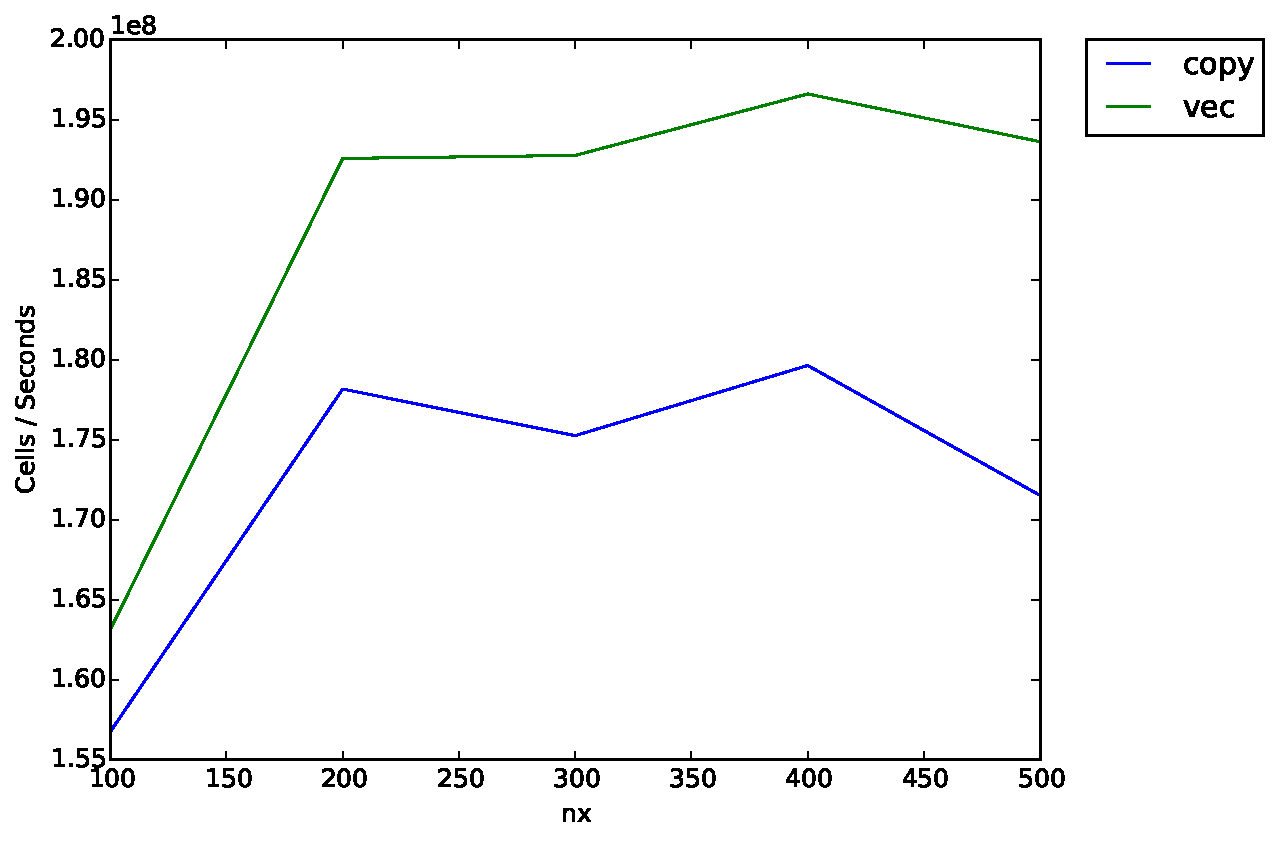
\includegraphics[width=0.8\textwidth]{figs/vec-timing1.pdf}
    \caption{Vector Timing Result ($cells/seconds$ vs. $nx$)}
    \label{fig:vector_timing_result1}
\end{figure}

\begin{figure}[h]
    \centering
    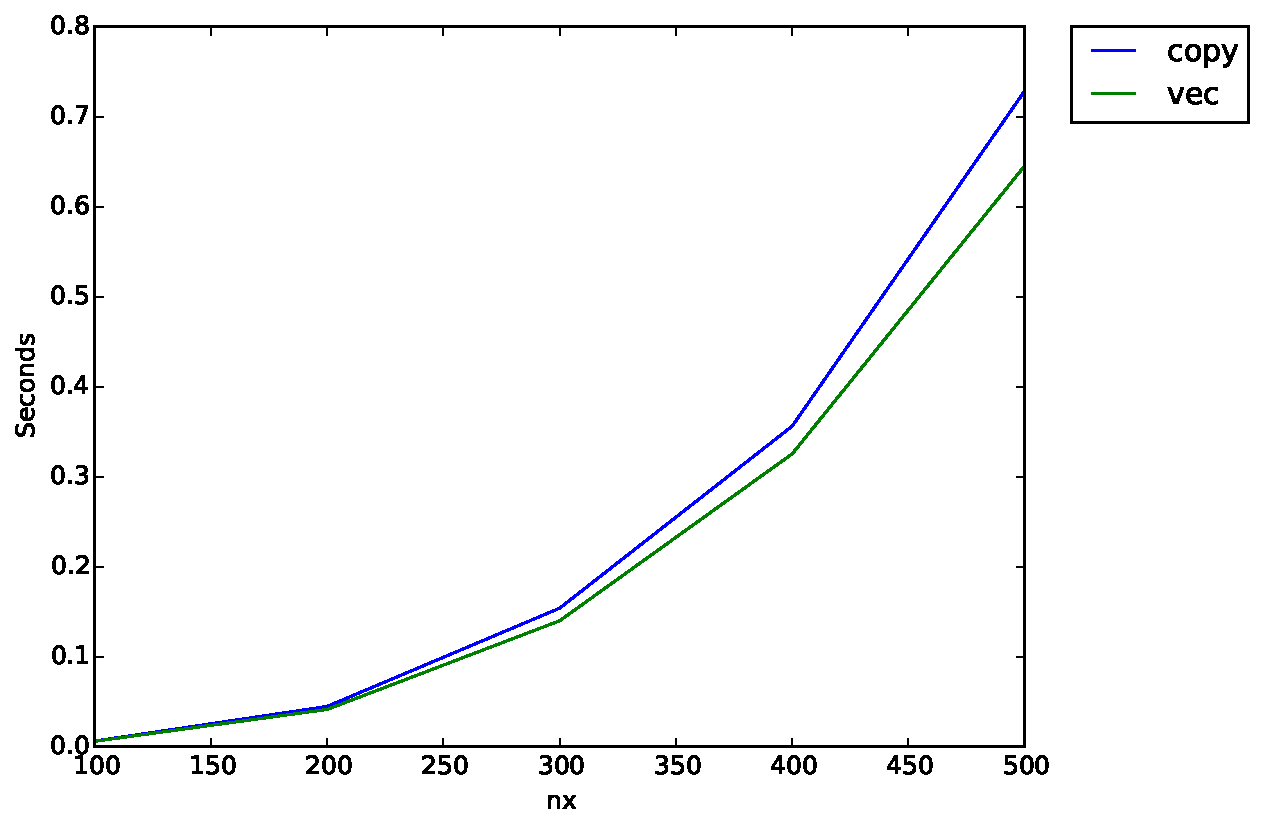
\includegraphics[width=0.8\textwidth]{figs/vec-timing2.pdf}
    \caption{Vector Timing Result ($seconds$ vs. $nx$)}
    \label{fig:vector_timing_result2}
\end{figure}

\subsection{What Worked}
We swept nx from 100 to 500 to see how the performance works given $nx$. First, like we have mentioned above, we could see timing is proportional to $ nx^{3} $. In terms of performance improvement, we could achieve quite good improvement by just doing vectorization. If you see Figure ~\ref{fig:vector_timing_result1}, vectorization did more jobs per second. 

\subsection{What did not work}
We tried OpenMP to make it parallel. Like we said at earlier section, OpenMP is a powerful tool to use to increase performance, but we noticed that it actually decreases the performance. Since it exceeded wall clock time, we could not even get the result yet. Hopefully, after the feedback, we can work on parallel part again. 
